% !TeX root = ../main.tex
\chapter{研究现状}
\label{cha:relate}
第\ref{sec:pt-related}节中首先简要回顾了传统视觉模型预训练方法,包括基于图像分类的有监督方法和基于图像自身的自监督学习的方法。随后,第\ref{sec:vl-related}节介绍了基于自然语言监督的视觉表征学习方法及其训练数据研究,并详细分析了从早期方法到语言-图像对比学习方法的发展历程。在此基础上,第\ref{sec:clip-related}节深入讨论了语言-图像对比学习在视觉表征增强以及下游任务迁移等方面的研究现状。


\section{传统视觉模型预训练方法}
\label{sec:pt-related}
% 这里是否花点章节介绍Pre-CLIP之前的一些工作?
% 总:    重提一下计算机视觉的里程碑时刻ImageNet的提出时,已经有初步的设想(WordNet)通过文本来构建信号,但因为历史原因,最终还是用无序无语义的label index的分类进行建模,使用文本的很少。CC出现是一个很强的信号(Crowd VL Data),基于此VirTex/ICMLM是两个早期探索,说一下贡献和局限性。
% Ins-Tag
% CC,LocNar(细粒度的),还有UNSUPERVISED VISION-LANGUAGE GRAMMAR INDUCTION WITH SHARED STRUCTURE MODELING等
% VirTex,ICMLM

%%% 回顾历史,尽量不要太长(0.5-1页左右)
在基于自然语言监督的视觉表征学习方法出现之前,视觉模型预训练方法主要分为三类:基于图像分类的有监督方法、基于图像话题标签的弱监督方法和基于图像自身的自监督方法。这三种方法对语义信息的利用程度各不相同,在预训练数据的可扩展性上也存在差异,形成了视觉预训练的三个发展阶段。 % 而变革的底层驱动力来自于进一步增强方法的可扩展性。

% 有监督 重提WordNet,语义变label,卡住泛化性
% 弱监督 主要提Meta的Ins-Tag,label变tag,domain狭窄
% 自监督 一次转向,抛弃任何语义信号的监督,回到视觉模型预训练本身

% 这里其实可以画个图
% 在视觉模型预训练方法研究早期,已有不少研究工作探索使用有语义的训练信号来监督视觉模型训练的方法\cite{devise},但长久以来并未找到足够高效,且可扩展性较强的方式。
视觉模型预训练方法的第一个发展阶段的里程碑是提出了ImageNet数据集\cite{deng2009imagenet}。以此为基础,基于图像分类任务的有监督预训练方法\cite{alexnet,resnet,googlenet,densenet}得到了飞速发展。
ImageNet数据集是基于词汇网络\cite{miller1995wordnet}(WordNet)构建的。词汇网络建立了各类单词与概念之间的知识图谱关系,而ImageNet数据集则从中选取部分名词概念,通过搜索引擎收集并经人工校验,为每个类别整理了相应的图片集合。
基于图像分类任务的有监督预训练方法将每类图片对应为一个类别序号,并限制模型需要识别的总类别数目。比如,常用的ImageNet-1K子集上的图像分类任务构建了1000个最常见类别集合进行图像识别训练。
这种预训练方法虽然使用了包含语义信号的训练数据,但在方法建模上并未直接使用类别标签自带的语义信息。因此,这种预训练方法在跨类别集合识别任务上的泛化效果不佳\cite{imagnettransfer},无法处理开放集合图像识别问题。此外,图像分类数据集的构造成本较高,因此常见数据集至多包含千万级别图片,可扩展性不佳。
虽然有不少工作尝试将这种基于图像分类任务的预训练方法进行大规模扩展,比如谷歌公司的JFT-300M\cite{Sun_2017_JFT300m}和JFT-3B\cite{zhai2022scaling}数据集。这些数据集促进了Transformer模型结构\cite{Transformer}在视觉领域中的应用\cite{dosovitskiy2020vit, coatnet},并推动了这类模型结构的进一步扩展\cite{zhai2022scaling, vit22b}。但由于隐私政策、商业考虑等各类原因,这些后续工作所提出的数据集和模型均未开源,相关学术成果也无法复现或使用。

为了扩展可用预训练数据来源,提升模型的泛化效果,研究者提出了弱监督预训练方法,其中代表性工作是IG-3.5B数据集\cite{mahajan2018exploring}。该数据集采用了照片墙应用(Instagram)上数十亿公开图片作为数据源,以用户添加的话题标签(Hashtag)作为图像标注。
这项工作开创性地使用了大规模标注有噪声的图像数据进行预训练,也将ImageNet数据集的单类别识别问题拓展为多类别识别问题,增加了预训练阶段的训练信号。
但与基于图像分类任务的有监督预训练方法类似,基于图像话题标签的弱监督预训练方法仍然将话题标签映射为固定集合内的类别序号,并不直接利用标注中的语义信息,因此这种方法的视觉表征语义能力较弱,跨类别集合的泛化性欠佳。
此外,这两类预训练方法都局限于固定类别集合的分类问题,因此训练信号较为稀疏。以ImageNet数据集为例,其包含了21841个不同的图像类别,每个类别序号仅能为单个图像样本提供约14比特的训练信息。在更常用的ImageNet-1K子集中,这一数值进一步缩小,只有约10比特。因此,这些预训练方法容易出现模型过拟合问题,限制了预训练模型的泛化性。

% 弱监督预训练方法拓展了视觉模型训练信号的来源。IG-3.5B数据集\cite{mahajan2018exploring}利用了脸书公司旗下的产品进行数据收集,将原先有监督预训练方法使用的单类别概念推广至任何与图像相关的话题标签(Hashtag)。另一类弱监督预训练方法则利用模型自己标注、自己训练的自举方法来增加监督信号来源\cite{yalniz2019billionscalesemisupervisedlearningimage,softteacher,mixedtraining},因此也被称为半监督训练方法。
% 但不管是利用话题标签作为标注或模型自主生成标注的方法,弱监督预训练过程中监督信号的语义信息始终有限。

为了进一步增加预训练阶段可用的训练数据,基于图像自身的自监督预训练方法放弃了难以建模和获取的语义信号,转而挖掘图像自身信息进行自我监督学习,使得预训练阶段的可用数据量在理论上可以无限扩展。
基于图像自身约束的自监督预训练方法有两个成功应用,分别是以SimCLR方法\cite{chen2020simple}为代表的对比学习预训练方法,和以MAE方法\cite{he2022masked}为代表的掩码图像模型预训练方法。前者方法利用图像的空间连续性、平移不变性等假设,要求模型识别两张数据增强后的图像是否属于同一原始图像\cite{moco,byol,dino},而后者则受自然语言处理领域发展\cite{BERT,gpt2}和Transformer模型结构在视觉领域应用\cite{dosovitskiy2020vit}的影响,强调关注图像作为二维信号的内部上下文关系,要求模型通过被掩码的部分图像恢复出完整的原始图像或特征图\cite{ImageGPT,bao2021beit,xie2022simmim,baevski2022data2vec}。
由于这些方法利用图像自身约束构造了更丰富的训练信号,比如对比学习方法的训练信息量与数据集中图像实例数目正相关,在常见数据集中为20至30比特;而掩码图像模型的训练信息量与图像分辨率正相关,通常包含$10^6$至$10^7$比特。因此,这些方法不容易出现预训练过拟合的问题,可以驱动大规模模型训练。
但是,由于自监督预训练方法在预训练过程中不使用任何语义信息,因此其依赖额外的视觉表征与语言表征的对齐阶段使得模型完成从感知特征到语义概念的映射。
此外,虽然自监督预训练方法的理论训练信号非常丰富,但由于这些训练信号侧重低级感知能力,多样性不足且不包含语义信息,因此这种预训练方法的数据利用效率并不高\cite{SEER, xie2023data},限制了此类方法的进一步扩展。

% 自监督预训练方法利用图像自身约束作为视觉模型训练信号的来源。实例级自监督方法以MoCo\cite{moco}和SimCLR\cite{chen2020simple}为代表性工作,其核心思想是将同一图像的不同视图视作对同一抽象对象的不同描述,或称为正样本对,而将不同图像的不同视图视作负样本对。MoCo\cite{moco}方法通过动态字典维护负样本对,而SimCLR\cite{chen2020simple}方法将其简化,只依赖当前批内图像作为负样本对。后续的代表性工作,如BYOL\cite{byol}和DINO\cite{dino},则使用双网络分支和特征一致性损失消除了对实例级对比方法中负样本的依赖。% 都是sg-ema+online,不对称结构,BYOL是ResNet+MSE,DINo是ViT+-plogq;https://blog.csdn.net/qq_56591814/article/details/127564330
% 另一类自监督预训练方法则是利用原始图像或特征图像素级别监督的像素级自监督方法。此类方法深受自然语言处理领域\cite{BERT,gpt2}发展和Transformer模型结构在视觉领域应用\cite{dosovitskiy2020vit}的影响。ImageGPT\cite{ImageGPT}和BEiT\cite{bao2021beit}受掩码语言建模方法\cite{BERT}启发,分别利用像素空间聚类和离散变分自编码器\cite{dVAE}的方式对图像进行标记化后进行序列掩码建模。后续的工作则进一步简化,通过回归损失消除了对图像标记化步骤的依赖。MAE和SimMIM\cite{he2022masked, xie2022simmim}方法提出通过掩码图像直接预测原始像素作为预训练的代理任务。Data2Vec\cite{baevski2022data2vec}方法则扩展了DINO\cite{dino}等双网络分支的工作,利用掩码图像的特征图一致性作为监督信号。这种方法与知识蒸馏\cite{deit,hinton2015knowledge}有相似的思想,也启发了本文第\ref{cha:fd}章的工作。

% 以vision model出发的一些历史回顾;1.2.1主要列了思想和代表性工作,这里要把更多相关工作给引入进来(1页以内)
% 这里可以仿照达哥做一个图;但主要担心是和1.2.1 写得太像。
% 有监督的imagenet,jft300m(Sun_2017_JFT300m),jft3b;scale vit(zhai2022scaling),vit22b

\section{基于自然语言监督的视觉表征学习方法}
\label{sec:vl-related}
% 视觉-语言多模态预训练方法主要分为两类。第一类方法被称为视觉-语言多模态融合方法。这类方法从已经预训练好的视觉模型和语言模型出发,通过引入额外的模型结构和代理任务对视觉表征和语言表征进行融合。
% % 并利用前文提到的互联网\{图像,替代文本\}对数据\cite{YFCC100M, sharma-etal-2018-conceptual, changpinyo2021conceptual}进行学习。
% 第二类方法被称为视觉-语言多模态联合预训练方法,包括本文的主要研究对象语言-图像对比学习预训练方法。这类方法从预训练阶段就考虑了视觉表征和语言表征的对齐与融合问题,通过视觉信息和语言信息互相监督的方式,使其天然具有处理视觉信息与语言信息的能力。
相比传统视觉模型预训练方法,基于自然语言监督的视觉表征学习方法直接利用文本描述中的丰富语义信息驱动视觉表征学习。本节将从训练数据构建和训练方法两个方面,分析这类方法的发展历程。% 特别地,我们将重点关注从早期的密集图像描述数据集,到近期的大规模图文数据集的演进过程,以及从基于文本生成的预训练方法到语言-图像对比学习方法的技术进展。

\subsection{训练数据研究}
%%% 引出基于语言监督的视觉模型训练的重要工作(0.5-1页左右)
% 分析主要目标等等
% 主要推动力:data
% \todo{图:有监督、弱监督、自监督、语言监督(vg,caption)}
% 得益于自然语言处理领域的最新进展\cite{Transformer,BERT,gpt2,elmo},视觉-语言多模态联合预训练方法登上历史舞台。站在视觉模型预训练的角度,视觉-语言多模态联合预训练方法本质上是利用语言信号为视觉模型提供监督信息。
数据驱动是“预训练-微调”范式的核心理念之一。基于自然语言监督的视觉表征学习方法的发展,与其训练数据形式的演进密不可分。
% 得益于自然语言处理领域的最新进展\cite{Transformer,BERT,gpt2,elmo},相比于第\ref{sec:pt-related}节中介绍的三种视觉模型预训练办法。
% 视觉-语言多模态预训练方法的核心是对数据中的语义信息进行充分挖掘和建模,其本质是用语言信号驱动视觉模型训练。
% 相比于使用图像类别序号作为训练信号的有监督方法和弱监督方法,视觉-语言多模态预训练方法可利用的语义信息内容更加丰富、形式更加多样、描述粒度更全面。

% 将视觉模型的监督信号从用类别序号表示的名词概念或者话题标签,推广到内容多样更强、描述粒度更细的自然语言信号。
% 因此此类方法在直接利用语义信息作为监督的同时,提升了监督信号的泛化性和所蕴含的信息量。
Visual Genome\cite{krishna2017visual}是基于自然语言监督的视觉预训练数据构建方法的重要代表。该方法提出稠密图像标注的概念,为每张图像标注了对象信息、属性特征、位置信息和相对关系等各类内容,并将这些信息用自然语言表示作为预训练信号。这种方法也启发了后续的稠密图像描述任务和多模态大模型与人类意图对齐任务\cite{imageinwords,flexcap,densecap}。
但这类方法的训练信号建模复杂,标注成本高,限制了训练数据样本的可扩展性,不适合作为大规模预训练数据构造方法。
因此,数据获取更容易、可扩展性更好的互联网图文数据对构建方法\cite{YFCC100M, sharma-etal-2018-conceptual, changpinyo2021conceptual}逐步替代了基于稠密图像标注的数据构造方法。
互联网图文数据对构建方法创新地利用网页代码中描述图像内容的文本属性,来构建视觉信息与语言信息配对的训练数据。得益于互联网技术的普及和用户生成内容的广泛应用,这类图文数据对通常具有千万甚至亿级规模,具有获取成本低、数据多样性好的优势。
虽然互联网图文数据对不如稠密图像标注数据的语义信息含量高,同时受数据噪声干扰较大,但由于其出色的数据可扩展性,使得这类数据构造方法已经成为主流的训练数据获取方法,为后续相关工作的发展奠定了基础。

然而,互联网图文数据对构建方法也面临两个主要挑战:首先,互联网数据缺乏质量控制和规范标准,存在大量噪声数据;其次,开源的图文数据集规模较小,限制了相关研究的进一步开展。
为解决这些问题,研究界在提升预训练数据质量和开源更大规模数据集等方面提出了诸多工作。
YFCC\cite{YFCC100M}和Conceptual Captions系列\cite{sharma-etal-2018-conceptual,changpinyo2021conceptual}工作率先开源了较大规模的互联网图文数据对,并提出通过图像分辨率和长宽比、文本长度和规范度等多维度人工规则来过滤低质量数据。但这类早期数据集的规模通常仅有千万级别,难以满足大规模预训练的需求。
由于互联网开源项目Common Crawl\cite{cc}提供了海量网页数据资源,因此LAION等工作\cite{schuhmann2021laion400m,schuhmann2022laion5bopenlargescaledataset,COYO-700m}从中构建并开源了更大规模的数据集,将规模从亿级扩展到十亿级,并创新地利用预训练好的语言-图像对比学习模型来评估和筛选高质量的图文数据对。DataComp工作\cite{datacomp}则基于LAION的开源数据集,构建了对比数据质量筛选方式优劣的评测基准。
MetaCLIP\cite{xu2024demystifying}工作则从更深层次探讨了数据质量问题。该工作遵循OpenAI CLIP工作\cite{radford2021learning}的数据构建方法,从文本N元语法分布的角度优化概念的多样性和均衡性,有效提升了数据集中独特语义信息的覆盖率。
此外,一些研究开始探索新的数据组织形式。MM-C4\cite{MM-C4}和OBELICS\cite{OBELICS}等工作提出了多图像多文本的交错图文对形式,以期通过更复杂的对应关系提供更丰富的语义信息。

% (Alternative Text,简称为Alt-Text)作为低成本、富语义、高多样性的自然语言监督信号,驱动视觉模型预训练。
% 替代文本本身是一种在网页代码中用于描述图像内容的文本属性。当图像无法显示时,浏览器会显示这些替代文本。因此这些替代文本常被用于帮助视觉失能用户理解图像内容,或被搜索引擎用于优化图文检索系统。
% 这类语义信号虽然不如Visual Genome方法所标注的内容信息含量高,也存在大量噪声问题。但由于互联网多年发展的积累,这类文本往往以千万甚至亿级别的规模存在,而且与图像成对出现,形成天然的\{数据,标注\}配对。


\subsection{训练方法研究} %{视觉-语言多模态模型模态对齐训练方法}
% \subsection{视觉-语言多模态联合预训练方法} %\paragraph{视觉-语言多模态模型联合预训练方法}
% % 先介绍一点VirTex相关的
% % 再介绍CLIP
% % 再介绍CLIP++
% 与视觉-语言多模态融合方法不同,视觉-语言多模态联合预训练方法不依赖单模态预训练的视觉模型和语言模型,相反地,这类方法从预训练阶段就通过视觉信息和语言信息互相监督训练的方式,实现了不同模态表征的融合,无需额外的模态表征融合阶段。
基于自然语言监督的视觉表征学习方法的核心是对数据中的语义信息进行充分挖掘和利用,从而驱动视觉模型训练。
% 相比于使用图像类别序号作为训练信号的有监督方法和弱监督方法,视觉-语言多模态预训练方法可利用的语义信息内容更加丰富、形式更加多样、描述粒度更全面。

如第\ref{sec:clip-introduce}节中所述,早期基于自然语言监督的视觉表征学习方法主要受自然语言处理领域启发:以图像为条件的掩码语言模型\cite{sariyildiz2020learning}继承了掩码语言模型\cite{BERT}(BERT)的掩码预测思想,而从文本标注中学习视觉表征方法\cite{desai2021virtex}则采用了生成式语言模型\cite{gpt2}(GPT)的自回归设计。
受限于较低的掩码比例,掩码语言模型的训练信号较为稀疏,训练效率不高。相比之下,生成式语言模型的自回归设计基于马尔可夫性质,将文本序列的联合概率分解为单文本标记预测的条件概率乘积,能够充分利用完整的语言信息。这种方法在训练单文本标记预测任务时都依赖正确的前序文本(即“教师强制”策略),因此训练效率更高。
然而,尝试将从文本标注中学习视觉表征方法扩展到更大规模时,研究者遇到了重要挑战:这类方法假设图像与文本存在严格对应关系,这与互联网图文数据对中普遍存在的噪声特性不相符。
为解决这一问题,研究者提出了两种改进方案:前缀语言模型\cite{SimVLM}(PrefixLM)和序列到序列模型\cite{GIT}(Seq2Seq)。这些变体将部分文本内容从训练目标转换为输入条件,放松了图像与文本强对应约束,从而在训练效率和数据可扩展性之间取得了更好的平衡。为了进一步放宽图像与文本严格匹配的数据假设,研究者开始探索另一种范式,即语言-图像对比学习方法,来优化视觉与语言表征间的相对关系。

% 此外,这些方法比较适合迁移到依赖多模态表征融合的下游任务,但在单模态下游任务上的微调表现欠佳。

% 以图像为条件的掩码语言模型\cite{sariyildiz2020learning}是早期代表性的视觉-语言多模态预训练方法。这种方法是自然语言处理领域中的掩码语言模型\cite{BERT}的扩展。具体而言,给定一条配对的图像与文本数据,该方法首先随机选择一定比例的文字用一个特殊的掩码词元进行替换,其次要求模型利用图像信息,预测被替换的文字的原始内容。
% 这里将可训练模型参数记为$\theta$,将图像信息记作$I$,并将长度为$n$的文本序列记作$T=\{t_1,\cdots ,t_n\}$。以图像为条件的掩码语言模型预训练方法在最大化如下概率估计:
% \begin{equation}
%     \max_{\theta}\sum_{t_i\in T'}\log\left({p_{\theta}(t_i|T-T',I)}\right),  
%     \label{eq:icmlm}
% \end{equation}
% 其中$T'$为被替换成掩码词元的部分文字集合,$T-T'$表示文本序列中未被替换成掩码词元的文字集合。这种视觉-语言多模态预训练方法和掩码语言模型类似,只会对长度为$n$的文本序列进行部分掩码训练。通常的掩码比例为15\%。因此针对每条图文对训练数据,该方法只能借助其中一小部分语义信息来驱动模型训练。

% 从文本标注中学习视觉表征方法\cite{desai2021virtex}的出现正是为了在模型预训练过程中尽可能利用更多的语义信息进行学习。这种方法同样受自然语言处理领域的发展启发,是自回归语言模型\cite{gpt2}在视觉-语言多模态预训练方向的扩展。
% 与以图像为条件的掩码语言模型方法不同,从文本标注中学习视觉表征方法要求模型利用图像信息,预测对应文本的完整文字序列。虽然从理论上而言,将以图像为条件的掩码语言模型方法中的掩码比例设置为100\%,即可驱动模型去预测完整文字序列,但这个预训练任务难度过高,几乎无法提供有意义的学习方向。
% 为解决这一问题,从文本标注中学习视觉表征方法借鉴了自回归语言模型中的马尔可夫性思想。将文本从左往右的书写顺序理解为系统的前后状态,而马尔可夫性质决定了系统的下一状态只依赖于当前状态,因此,文本序列的生成过程可以被拆分为从左往右的迭代过程。
% 与式\eqref{eq:icmlm}中符号一致,从文本标注中学习视觉表征方法在最大化如下概率估计:
% \begin{equation}
%     \max_{\theta}\sum_{i=1}^{n}\log\left({p_{\theta}(t_i|t_{1:i-1},I)}\right)    
%     = \max_{\theta}\log\left({p_{\theta}(t_{1:n}|I)}\right),
%     \label{eq:character-level}
% \end{equation}
% 其中$t_{1:0}$可以理解为空序列。可以看出,从文本标注中学习视觉表征方法通过马尔可夫性,将基于图像信息的文本序列预测任务拆分成了多个单文字预测任务,并在每个单文字预测任务中都基于正确的前序文本序列进行预测。这种思想也被称为“教师强制”(Teacher Forcing)。
% % https://www.cnblogs.com/dangui/p/14690919.html
% 通过这种方式,从文本标注中学习视觉表征方法可以充分利用每条图文对训练数据中的语义信息进行模型预训练,进一步增强了模型对语义信息的建模能力。相比于以图像为条件的掩码语言模型预训练方法,这种方法得到的视觉模型在各类下游任务上的迁移效果更佳。

% 早期视觉-语言多模态模型联合预训练方法主要是扩展了掩码语言标记建模BERT模型\cite{BERT}和基于自回归语言建模的GPT模型\cite{gpt2}。
% 前者以ICMLM方法\cite{sariyildiz2020learning}为代表。这种方法利用\{图像,文本\}配对数据完成基于图像内容的掩码语言标记建模。通常而言,每一条输入文本的15\%的词会被随机掩码。因为文本内容的冗余性比较低,信号具有离散性,因此掩码标记无法提供除占位信息之外的任何内容。这一点也在第\ref{chap:ddcap}章所讨论。这一特点导致掩码比例无法被扩展到一个较大的值\cite{BERT, BERTmask}。
% 有限的掩码比例导致这类方法的单样本训练信号较少,学习效率并不高,后续逐渐被以VirTex\cite{desai2021virtex}为代表的基于自回归语言建模的工作所取代。基于自回归的方法建模了整条样本的联合概率分布,训练信号丰富,是大规模扩展工作的主要思路\cite{SimVLM, GIT},并延伸出前缀语言模型\cite{SimVLM}和序列到序列模型\cite{GIT}两种变体。
% 但这些后续工作以完成视觉-语言多模态下游任务为主,未讨论过其视觉模型的迁移效果,也无法将其用于大规模图文检索系统。
% 此外,如节\ref{sec:instance-purpose}中的分析,此类方法建模了图像与文本的强对应关系,对数据质量要求较高,这也是GiT\cite{GIT}方法仅用一半数据就超过SimVLM\cite{SimVLM}方法的重要原因之一。


\begin{figure}
  \centering
  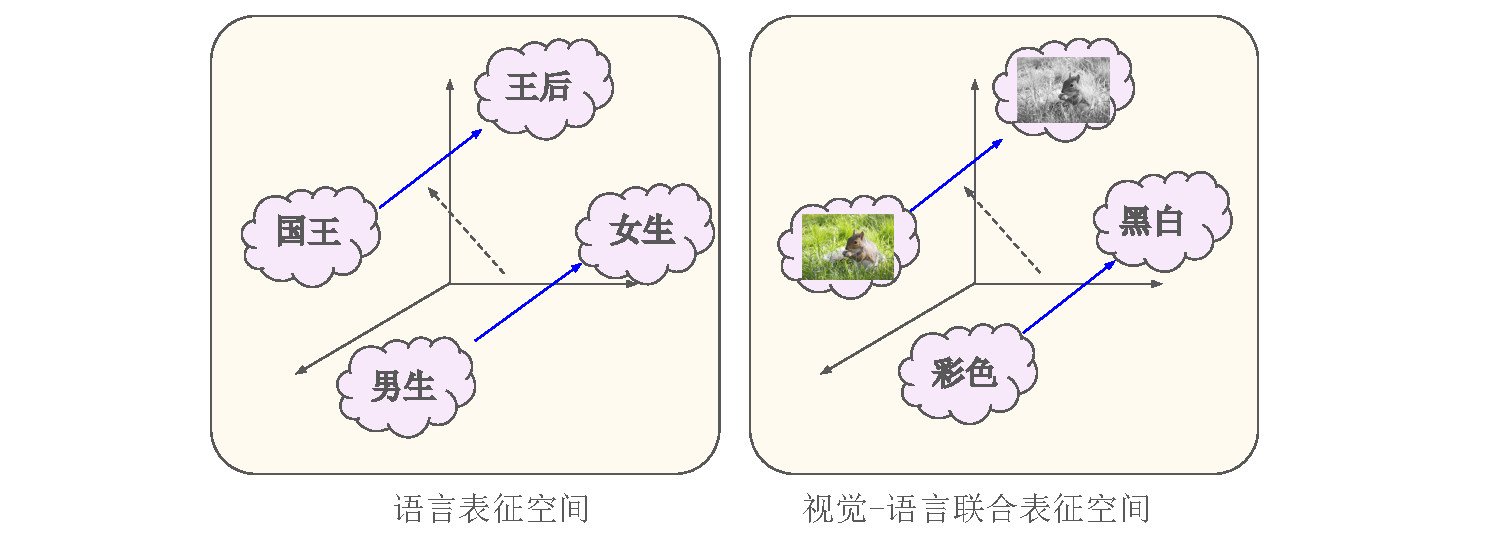
\includegraphics[width=1.0\linewidth]{figures/论文-CLIP性质-v2.pdf}
  \caption{语言表征空间与视觉-语言联合表征空间的相似性示意图}
  \label{fig:clip-word2vec}
\end{figure}

语言-图像对比学习(CLIP)方法\cite{radford2021learning,jia2021scaling,pham2023combined}借鉴了实例级对比学习自监督方法的思想,将视觉表征的预训练任务从“预测语言信息”转变为“与语言表征对齐”。这种多模态对比学习策略通过建模不同模态表征间的相对距离,有效降低了对图像与文本严格对应关系的依赖。同时通过构建视觉-语言联合表征空间,CLIP方法能够驱动模型学习更具判别性的表征,从而提升了模型在下游视觉任务上的迁移效果。
更重要的是,CLIP方法构建的视觉-语言联合表征空间具有独特的性质,使得CLIP方法特别适合用于模态表征提取和跨模态表征转换与检索等任务。
视觉-语言联合表征空间的性质与语言表征空间\cite{word2vec,distword2vec}有相似之处。如图\ref{fig:clip-word2vec}左侧所示,在语言表征空间中,不同概念的表征之间存在可解释的线性关系。例如,“女生”的表征减去“男生”的表征,再加上“国王”的表征,可以得到“王后”对应的表征。
CLIP方法构建的联合表征空间也展现出类似的线性关系。如图\ref{fig:clip-word2vec}右侧所示,通过“黑白”语言表征减去“彩色”语言表征,可以获得表示颜色变换的向量,再将这个向量应用到彩色图片的视觉表征上,就能有效检索到对应黑白图像的视觉表征。
这种多模态表征对齐能力不仅使得CLIP方法在图文跨模态检索任务上表现优异,还表明CLIP方法习得的视觉表征中包含了丰富的语义信息,为开放集合图像识别任务的发展提供了重要基础。

% 将自监督预训练方法\cite{moco, chen2020simple}的正负样本对思想引入视觉-语言多模态训练中。
% 视觉模型自监督预训练工作本质上将同一图像的不同视图视为对某一抽象对象的不同描述。自监督对比学习的核心思想正是建模关于此抽象对象的不变表征。
% 将这一思想推广到\{图像,文本\}配对数据后,CLIP方法将图像和文本分别理解为某一抽象对象的不同描述,因此配对的图像和文本可以被视作正样本对,而任一不配对的图像与文本均被视作负样本对。% 这写的不是车轱辘话?

\section{语言-图像对比学习方法}
\label{sec:clip-related}
作为一种重要的“预训练-微调”方法,CLIP方法的相关研究主要关注如何提升预训练阶段的可扩展性,增强其视觉表征的语义建模能力,同时提升CLIP方法在多种下游任务中迁移表现和泛化性。

\subsection{视觉表征学习增强方法研究}
% 泛化能力\cite{ftclip2021, clip-generalize, languagehelpvision, clipshortcut}
% 预训练效果\cite{li2022supervision,TCL,SLIP,MaskCLIP,CoCa,EVA,pham2023combined,pali,LiMoE,palix}
% 可以recall 目标
% 如前文所述,预训练阶段是整个“预训练-微调”范式的核心。因此如何进一步提高语言-图像对比学习方法的预训练可扩展性,增强视觉表征与语言表征的对齐效果是重要研究目标之一。各类工作围绕如何高效扩展预训练数据和模型参数规模,以及如何进一步增加预训练信号的来源,降低预训练数据噪声干扰展开了系列研究。
预训练阶段是整个“预训练-微调”范式的核心。因此,进一步扩展CLIP方法、增强其视觉表征的语义建模能力、提高视觉表征与语言表征的对齐效果,是该领域的重要研究方向。现有工作主要围绕扩展预训练数据和模型规模、降低预训练成本与代价、拓宽预训练信号来源以及分析模型特征属性展开。

\paragraph{扩展预训练数据与模型规模} 由于CLIP方法具备大规模扩展的潜力,因此许多研究致力于进一步提升其可扩展性。
BASIC方法\cite{pham2023combined}从工程优化角度,提升了CLIP方法的可用数据规模、模型参数数量和训练批次大小。相比于最初的OpenAI CLIP方法\cite{radford2021learning},BASIC方法采用的训练数据规模扩大了16倍,视觉模型参数增加了4倍,训练批次大小增大了4倍,充分展示了CLIP方法的可扩展性。
PaLI系列方法\cite{pali,palix}不仅进一步提升了视觉模型的参数规模,还结合大语言模型提升了CLIP方法对语言信息的建模能力。此外,PaLI方法将以英文为主的互联网图文数据对扩展至覆盖100多种语言的图文数据对,显著增强了CLIP方法在跨语言任务上的泛化能力。
LiMoE方法\cite{LiMoE}引入混合专家\cite{gshard}(Mixture of Experts)模型结构,分别为视觉模态和语言模态设计独立的专家模型。在显著提升CLIP方法模型参数规模的同时,LiMoE方法通过部分参数激活的方式降低了计算成本,使得训练更加高效。

% 引入知识蒸馏方法
\paragraph{构建高效轻量的CLIP方法}
% 虽然这些方法在增强CLIP方法的预训练效果上取得了印象深刻的表现,但这些大规模的数据和模型一方面并未开源以推动研究进展。
随着CLIP方法预训练规模的不断扩大,其对大规模计算资源的依赖日益增加。高昂的训练成本限制了许多研究机构开展相关工作,因此提高预训练效率,降低预训练成本成为重要研究方向。CLIPA系列方法\cite{CLIPA,CLIPA-v2}提出了“逆扩展定律”:训练的模型参数量越大,所需的输入图像分辨率和文本序列长度越小,因此这一发现有助于降低预训练的计算开销。A-CLIP系列方法\cite{ACLIP,FLIP}则借鉴了自监督方法中的掩码图像模型思想,对输入图像进行部分掩码来减少训练过程中的计算开销。
此外,MobileCLIP\cite{MobileCLIP}和TinyCLIP\cite{TinyCLIP}等工作采用知识蒸馏方法\cite{hinton2015knowledge}来构建小规模模型,降低了CLIP方法在应用中的成本。

知识蒸馏方法\cite{hinton2015knowledge,kim2018paraphrasing}最早被应用于卷积神经网络中,后来被成功推广到Transformer模型结构\cite{deit,wang2020minilm}。这种方法的核心在于将教师模型的知识迁移到更小的学生模型中,因此,知识蒸馏是一种常用的模型压缩手段。研究表明,在图像分类任务中,当学生模型模仿教师模型的未归一化输出时,教师模型能够提供简单类别信息之外的“暗知识”\cite{furlanello2018born},从而提升学生模型的性能。% https://blog.csdn.net/Artistzq/article/details/125372542
除了在图像分类任务得以应用之外,知识蒸馏方法在深度强化学习\cite{chaudhry2018riemannian}、终身学习\cite{zhai2019lifelong}和推荐系统\cite{chen2018adversarial}等领域都取得了显著成果。
% 训练效率\cite{CLIPA,CLIPA-v2,MobileCLIP,VisionZIP,ACLIP,FLIP}

% 这个倒是可以画个图清楚一点
\paragraph{拓宽预训练信号来源与利用方式} 
除了通过扩大规模来改进CLIP方法,研究者还探索了在CLIP方法中引入其他训练信号的方式,以提高视觉表征的学习效果。
SLIP方法\cite{SLIP}借鉴了实例级自监督方法的思想,将CLIP方法与图像自监督对比学习方法\cite{chen2020simple}结合,增强了视觉表征的建模能力。DeCLIP方法\cite{li2022supervision}则在此基础上,进一步引入掩码语言模型来提升CLIP方法的语言建模能力,并通过图像增强和文本改写等技术构造更丰富的图文对齐数据。
受视觉-语言多模态训练方法\cite{visualbert}启发,TCL方法\cite{TCL}设计了多模态表征深度融合模块,通过图文配对预测任务来加强模态间的对齐效果。该任务在形式上与掩码语言模型的下一句子预测任务\cite{BERT}一致,加强了模型对图文关系的理解。MaskCLIP方法\cite{he2022masked}则结合了像素级自监督方法,在CLIP方法中引入掩码图像模型的训练任务\cite{he2022masked},从而进一步提升视觉模型对图像结构的感知能力。
CoCa方法\cite{CoCa}则在CLIP方法中重新加入从文本标注中学习视觉表征方法\cite{desai2021virtex},要求模型在对齐视觉表征和语言表征的同时,完成基于视觉表征预测输入文本内容的训练任务。最新提出的SigLIP-2方法\cite{siglip-2}更是整合了各类视觉和语言模型的自监督方法,以实现更好的单模态表征建模能力与跨模态表征对齐效果。

% 参考FD
\paragraph{模型特征属性诊断工具} 深度学习模型由于其高维和非线性特性,因此往往被视为“黑箱”系统。为了更好地理解模型的内部机制,模型特征属性诊断工具发挥着关键作用\cite{yosinski2014transferable}。这类研究不仅有助于解释模型的决策过程,也为模型设计和优化提供了重要指导。自Transformer模型结构提出以来,众多研究工作\cite{zhou2021deepvit, dosovitskiy2020vit, goh2021multimodal, dai-etal-2022-knowledge, imagnettransfer, raghu2021vision}致力于揭示其自注意力层和前馈层的工作原理。这些研究主要从以下几个方面展开:1)通过注意力机制分析方法\cite{zhou2021deepvit, dosovitskiy2020vit}可视化注意力权重分布,反映模型如何关注不同位置的输入,揭示模型的视觉感知偏好;2)通过损失景观可视化方法\cite{li2018visualizing}分析损失函数在模型参数空间中的分布特征,理解模型训练过程中的优化轨迹和收敛特性;3)通过层间相似度分析\cite{kornblith2019similarity}考察不同模型层表征间的相似程度,探究模型的层间结构化性质;4)通过知识神经元分析\cite{dai-etal-2022-knowledge, goh2021multimodal}识别模型中对特定概念异常敏感的神经元,揭示模型内部的知识表示方式。

现有工作在扩展预训练信号来源时,通常需要维护多个模型实例\cite{TCL,MaskCLIP}或处理多个图像增强视图\cite{SLIP,TCL,li2022supervision}。这种做法显著增加了预训练阶段的计算资源消耗。同时,现有的数据语义信号质量提升方法也存在局限性。基于启发式规则的筛选方法\cite{sharma-etal-2018-conceptual}可能误判数据质量,而依赖预训练模型打分的方法\cite{schuhmann2021laion400m}对细微质量差异的区分能力有限。
针对这些问题,本文第\ref{cha:iclip}章中提出了另一种研究方法,通过对比学习思想有效整合和深度利用了人工标注的图像分类数据源。这种方法不需要增强额外的模型参数或处理多个图像增强视图,利用高质量的图像分类数据提升了CLIP方法训练数据的整体质量,增强了CLIP方法的视觉表征学习效果。

% 第一点如何获取高质量图文的数据,并增加预训练信号来源是CLIP方法进一步扩展的关键因素。很多现有数据扩展工作并不开源,而数据收集的成本比较高,而且过滤方法需要人工规则,容易存在遗漏的情况,因此本文的第一项工作,就是基于低噪声图像分类数据增强的CLIP预训练方法。通过这种方法来加强视觉表征与语言表征的对齐,增强CLIP方法零样本图文跨模态检索和开放集合图像识别能力。
\subsection{下游任务迁移方式研究}
% 可以recall 目标
% 作为一种预训练方法,除了提升预训练阶段多模态表征对齐效果,提高语言-图像对比学习方法在各类下游任务上的迁移表现,并泛化到尽可能多的下游任务也是一个重要的研究目标。
作为一种预训练方法,CLIP方法的价值不仅体现在多模态表征的对齐效果上,更重要的是其迁移到下游任务后解决实际任务的能力。因此,提升CLIP方法在不同类型任务上的迁移性能并扩展其应用范围,也是该领域的重要研究方向。现有工作主要围绕开放集合识别的视觉任务、多模态语义生成任务以及多模态图像生成任务展开。

\paragraph{开放集合识别的视觉任务迁移}
% 迁移部分可以多加一些clip for zs seg/det这种工作
CLIP方法在零样本开放集合图像识别任务上展现出优异性能,这促使研究者探索将其开放集合识别能力迁移到更广泛的视觉任务中。
在目标检测任务中,ViLD\cite{ViLD}和F-VLM\cite{F-VLM}等方法将目标检测任务分解为定位和识别两个阶段,成功实现基于CLIP方法的开放集合目标检测任务迁移。这一思路启发了后续一系列工作\cite{Zhong_2022_CVPR, glip, detclip, detclip-2, detclip-3}。这些工作通过构建更细粒度的单词-区域对比学习方法,实现了真正意义上的开放集合目标检测能力。
在语义分割任务中,研究者致力于提取CLIP方法蕴含的像素级语义信息。相关工作\cite{denseclip, zsseg, openseg}主要采用两种策略:第一种策略是参考开放集合目标检测任务做法,将语义分割任务拆分为物体掩码预测和语义识别两个阶段;第二种策略是利用CLIP方法的视觉模型中的自注意力机制,聚合并提取属于同一类别的像素位置和语义信息。
此外,在少样本图像识别任务中,CoOp等工作\cite{coop,cocoop}通过引入提示微调等技术,显著提升了CLIP方法在精细类别图像识别任务上的迁移表现。
% 还有few-shot transfer的工作。

% 这个detclip竟然也讨论了dictionary enhancement的概念 for openvocabulary的det啊哈哈哈

\paragraph{多模态语义生成任务迁移}
% 图生文CLipCap;% 可以包括一些图像描述任务的讨论,以及之前放在2.2.2. 的视觉-语言多模态融合方法
% 还有后续的clip+llm的工作也可以写进来
% 语言-图像对比学习方法在预训练过程中允许模型同时理解视觉信息与语言信息,因此也非常适合迁移到多模态下游任务中。
% 视觉-语言多模态融合方法\cite{visualbert, vl-bert, uniter, OSCAR, VinVL, LEMON}本质上是一种两阶段的预训练方法。这类方法从已经预训练好的视觉模型和语言模型出发,通过引入额外的模型结构和代理任务对视觉表征和语言表征进行融合,再将得到的视觉-语言多模态模型迁移到各类下游任务中。
% 受掩码语言模型\cite{BERT}启发,这类方法往往把基于图像的掩码语言模型作为主要代理任务,并利用多模态数据特有性质来构建辅助代理任务,从而驱动视觉表征和语言表征融合。
多模态语义生成任务涵盖多个重要方向,包括图像描述生成\cite{vinyals2015show,karpathy2015deep}、视觉问答\cite{vqa}以及近期兴起的复杂人类指令理解任务\cite{llava}。其中,图像描述生成作为最基础的多模态语义生成任务,长期以来受到广泛关注。
早期的图像描述生成方法\cite{vinyals2015show,karpathy2015deep}采用卷积神经网络提取视觉特征,配合循环神经网络作为解码器生成图像描述。后期工作引入注意力机制提升了视觉和语言信息的融合效果\cite{huang2019attention,lu2017knowing}。为进一步提高图像描述生成任务效果,一些工作探索了利用语义属性\cite{yao2017boosting}和场景图\cite{yang2019auto}等额外信息的方法。受掩码语言模型的启发,研究者还尝试了非自回归方法\cite{gao2019masked}的图像描述生成迁移方法。这些技术进展不仅推动了图像描述生成任务的发展,也为其他多模态语义生成任务提供了重要借鉴。

早期的多模态语义生成任务迁移研究\cite{visualbert, vl-bert, uniter, OSCAR, VinVL, LEMON}主要基于单模态预训练的视觉模型和语言模型展开。这些方法通过引入额外的模型结构和多模态对齐任务,实现视觉和语言表征的深度融合。这类方法的典型做法是使用在Visual Genome数据集上微调的目标检测模型\cite{butd}作为视觉表征提取器,并将其提取的各区域特征输入到掩码语言模型中,完成以图像为条件的掩码建模任务。不同方法提出了多种创新性的辅助任务来增强模态融合效果。
% 早期多模态任务迁移方法从已经预训练好的视觉模型和语言模型出发,通过引入额外的模型结构和代理任务对视觉表征和语言表征进行融合从而迁移语义生成多模态任务中。这些方法通常使用在Visual Genome数据集上微调得到的目标检测模型\cite{butd}作为视觉特征提取器,再将其输入到掩码语言模型\cite{BERT}中,完成以图像为条件的掩码建模任务。不同方法引入了额外的辅助代理任务以增强模态融合的效果。
% VisualBERT方法\cite{visualbert}参考BERT\cite{BERT}方法中的下一句子预测任务,引入图文配对预测任务以增强实例级对应关系学习。VL-BERT方法\cite{vl-bert}为保留预训练语言模型的语言建模能力,避免预训练知识的灾难性问题\cite{catastrophic},在图文数据对之外加入纯文本数据进行补充。UNITER方法\cite{uniter}则参考文本的掩码建模任务形式,对物体检测框序列构造掩码区域特征建模任务,以增强视觉表征与语言表征的融合效果。Oscar方法\cite{OSCAR}除了将物体检测框对应的区域特征和区域位置输入语言模型之外,还将每个检测框的类别信息作为额外的输入信息,提供辅助融合信号。
由于目标检测模型作为视觉表征提取器存在两个主要问题:计算开销较大且检测框采样操作影响梯度回传,因此后续研究\cite{pixelbert, soho, vilt}提出了更高效的方案:直接使用视觉模型的特征图,或采用随机初始化的块嵌入层(Patch Embedding)作为视觉表征。这些改进为多模态语义生成任务迁移的端到端优化提供了可能性。
% 目标检测模型作为视觉表征提取器非常耗时,一些后续工作\cite{pixelbert, soho, vilt}提出使用视觉模型特征图或一个随机初始化的图像块投影层作为视觉表征输入到语言模型中,为端到端优化提供可能。

CLIP方法在预训练过程中实现对视觉和语言信息的双重理解,为多模态语义生成任务迁移提供了良好基础。一些工作\cite{song-etal-2022-clip, shen2022how}讨论了如何基于早期方法\cite{pixelbert}将CLIP方法的视觉模型迁移到视觉问答、视觉蕴含等多模态语义生成任务中。而CLIPScore方法\cite{CLIPScore}则创新地利用了CLIP方法多模态表征的对齐特性,构建了一个不依赖参考文本的图像描述生成质量评价指标。
近期,随着大语言模型的快速发展,多模态语义生成任务迁移研究出现了新的趋势。以BLIP-2\cite{blip-2}为代表的一系列工作\cite{minigpt4,llava,llavanextinterleave}探索了将预训练好的大语言模型与CLIP方法的视觉模型相结合的方法,充分利用了大语言模型的语义表达能力,开创了CLIP方法在多模态语义生成任务迁移的新方式。


\paragraph{多模态图像生成任务迁移}
CLIP方法对齐了视觉表征和语言表征,为多模态图像生成任务迁移提供了新的可能。其中,Dall-E 2方法\cite{dall-e2}开创性地利用了这种对齐特性实现CLIP方法在多模态图像生成任务上的迁移:该方法首先利用CLIP方法的语言模型得到输入文本的语言表征,然后训练一个基于扩散模型\cite{ddpm,ddim}的先验模型预测对应的CLIP视觉表征,最后再通过另一个扩散模型将CLIP视觉表征转化为实际图像。Dall-E 2方法在基于文本的图像生成任务中效果出色,在大量应用中得到应用。
作为Dall-E 2方法中的关键技术,扩散模型主要分为连续扩散模型和离散扩散模型两类。连续扩散模型\cite{beatsgan,ddpm,ddim,latentdiff}对连续的输入空间或特征空间进行建模,在基于文本的图像生成领域取得了显著成果,已发展成为主流技术路线。连续扩散模型的代表性工作包括GLIDE\cite{glide}、Imagen\cite{imagen}和Stable Diffusion\cite{latentdiff}等,在图像生成质量和可控性方面展现出优异表现。
相比之下,离散扩散模型的研究相对较少。ImageBART\cite{Imagebart}和VQ-Diffusion\cite{VQ-diffusion}等工作探索了在VQ-VAE\cite{dVAE,vqvae}方法构建的图像离散代码空间中应用扩散模型的可行性,为多模态图像生成任务迁移提供了新的解决思路。
% 对于文本生成,离散扩散仅在相对玩具的问题上显示出一些初步的成功 [3,26]。最近的工作 [41] 也尝试使用连续扩散进行文本生成,但更多的是用于细粒度的控制任务。

现有研究主要关注CLIP方法在对语义依赖程度较高的开放集合识别任务上的迁移应用,而对于需要密集感知能力的视觉任务的迁移方法研究较少。针对这一问题,本文第\ref{cha:fd}章提出了特征图自蒸馏方法。该方法无需重新预训练或额外数据标注,通过引入像素级视觉训练目标,显著提升了CLIP方法在细粒度视觉任务上的迁移性能。
在多模态语义生成任务方面,现有方法通常结合大语言模型并需要复杂的表征融合实现任务迁移,训练成本和系统复杂度都很高。为解决这一问题,本文第\ref{chap:ddcap}章探索了一种基于离散扩散模型的语义生成任务迁移方法,同时探讨了扩散模型在文本生成任务中的应用前景。
%%%%%%%%%%%%%%%%%%%%%%%%%%%%%%%%%%%%%%%%%%%%%%%%%%%%%%%%%%%%


% 达哥在讨论像素级任务的研究动机时起其实分析了实例级任务的缺陷(这部分可能会在我的前一部分讨论,前一部分讨论语言监督+基于掩码和自回归的两种细粒度办法;)
% 问题:什么时候提细粒度 data(以locnar为代表的)
% 先比较重要的两个工作:VirTex,ICMLM
% 分析贡献,讲述缺陷(数据获取难度,最大监督信号信噪比)
% 引出CLIP:介绍CLIP的具体做法,将其对比纯图像的实例级方法
% 针对之前讨论的非实例级的办法的缺陷,引出为什么这个办法好(合计1-1.5页左右)
% \begin{figure}
%   \centering
%   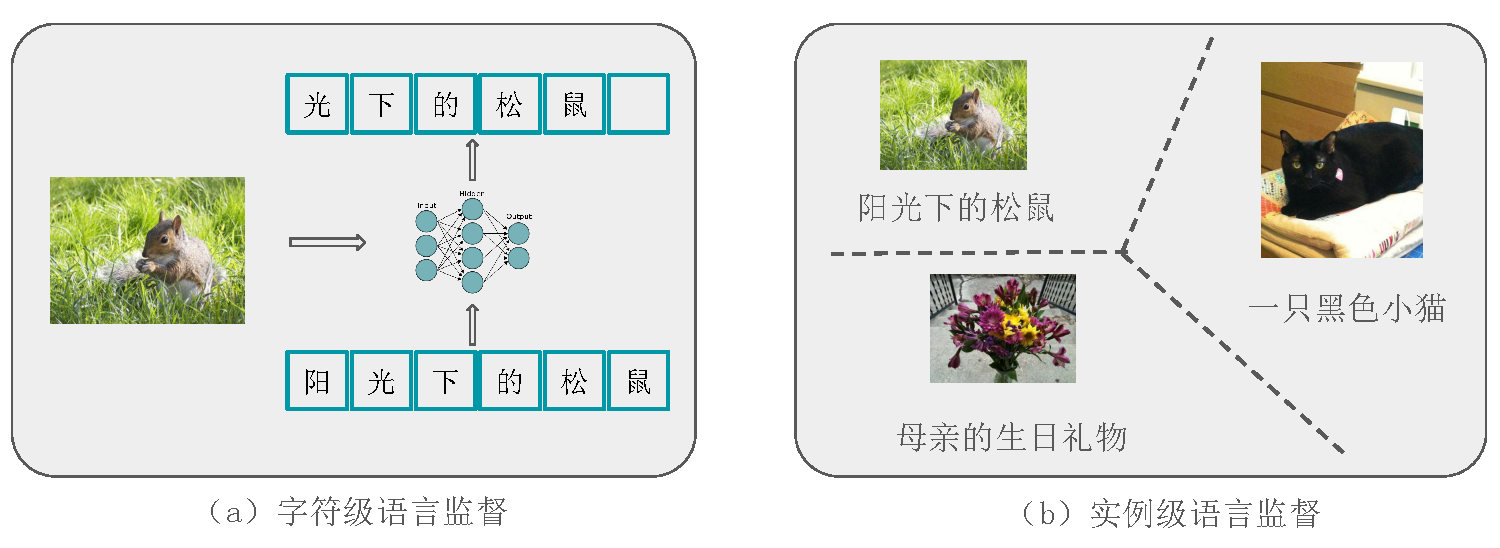
\includegraphics[width=1.0\linewidth]{figures/论文-图5-字符级-实例级.pdf}
%   \caption{字符级联合预训练方法和实例级联合预训练方法示意图}
%   \label{fig:5-character-instance}
% \end{figure}
% 如节\ref{sec:language-supervised}所述,站在视觉模型预训练的角度,视觉-语言多模态联合预训练方法本质是一种基于自然语言监督的视觉预训练方法。
% 与自监督视觉预训练方法的发展类似,基于自然语言监督的视觉预训练方法也有实例级别训练方法和更细粒度的字符级训练方法。但和自监督方法的发展历程有所区别,在实例级语言监督的方法出现之前,细粒度字符级监督方法占据主导地位。这类方法的核心思想是利用基于图像的文本生成任务作为预训练的代理任务,也即对任一给定的图像,训练模型去预测其对应替代文本中的任意字符。
% 延用之前对监督信号信息量分析的方法,较为流行的文本码本通常含有30000-100000个文本标记,而互联网中的替代文本平均长度约为20个标记,那么将这样的自然语言作为监督信号,信息量达到可观的300比特。同时监督信号信息量随着替代文本长度的增加而上升。

% 字符级联合预训练方法受自然语言处理领域的进展影响很大,其中两项代表工作分别是2020年提出的ICMLM\cite{sariyildiz2020learning}方法和2021年提出的VirTex\cite{desai2021virtex}方法。
% 两者分别是自然语言预训练方法中基于掩码语言标记建模模型BERT\cite{BERT}和基于语言自回归模型GPT\cite{gpt2}的拓展。其中基于自回归模型的VirTex方法(如图\ref{fig:5-character-instance}(a)所示)允许对自然语言监督信号进行充分利用,而ICMLM方法受限于掩码标记的比例不能过大,只能对监督信号的部分内容进行学习。因此基于自回归模型的方法在下游任务上的迁移表现普遍优于基于掩码语言标记建模的方法。
% 这些小规模的研究工作首次证明基于视觉-语言联合预训练方法得到的视觉模型在图像分类、目标检测等下游视觉任务上可以取得良好的性能表现,同时无需额外的模态对齐阶段即可完成诸如图像注释(Image Captioning)等多模态任务,初步展示出视觉-语言多模态联合预训练方法的巨大潜力。

% % 引出缺陷,引出CLIP,引出为什么CLIP好
% % 达哥的缺陷是先讲了自监督的目标(迁移性好,扩展性强),然后讲实例级这两方面不好(迁移性特指dense tasks)他是先从实例级做起的,然而我上来就是CLIP)
% 随着研究深入,字符级语言监督的训练方法弊端逐渐显现,其中的核心原因是这种训练方法对图文配对数据的质量要求较高。这里将图片记作$I$,将长度为$n$的字符标记序列记作$T=\{t_1,\cdots ,t_n\}$,记模型参数为$\theta$,字符级语言监督方法本质上在最大化如下概率估计:
% \begin{equation}
%     \max_{\theta}\sum_{i=2}^{n}log\left({p_{\theta}(t_i|t_{1:i-1},I)}\right)    
%     = \max_{\theta}log\left({p_{\theta}(t_{2:n}|t_1,I)}\right)
%     \label{eq:character-level}
% \end{equation}

% 因此,此类方法强化了图文对的对应关系,其优化目标最终导向图像与文本的一一配对。
% 然而,这个假设在现实场景中很难成立。一方面文本描述千变万化,本身不存在强对应关系,另一方面这也与互联网数据的特性有关。
% 互联网中的替代文本与弱监督方法中的话题标签类似,虽然大部分是人类所写,但其质量良莠不齐,容易出现占位符、无关文本或低信息文本的情况,标注的信噪比较低。
% 因此,前述提到的两种字符级语言监督预训练方法均只在噪声比例较低的\{图像,文本\}对数据集,如MSCOCO\cite{chen2015microsoft}数据集上有成功应用,难以推广到以互联网替代文本为主的更大规模数据集\cite{sharma-etal-2018-conceptual}。
% 这一点限制了此类方法的可扩展性和方法上限。
% % 缺陷2: 因为生成式的原因pt的时候难以跟踪模型分类性能?(knn/lp可以),有一点牵强。模型结构混合?和字符级监督没有本质关系。需要handle variance length?实例级为什么对这一点更效?
% % 其次,语言信号有天然的变长特性,因此字符级语言监督方法在“联合预训练”阶段存在不同(图像-文本)对训练不平衡问题,对应文本字符序列较短的图像存在学习不充分的现象。此外,字符序列长度不均衡也对算法实现效率带来了不少的挑战,这一点进一步限制了此类方法大规模扩展的有效性。

% \begin{figure}
%   \centering
%   \subcaptionbox{CLIP方法概览\label{fig:6-CLIP-Method}}
%     {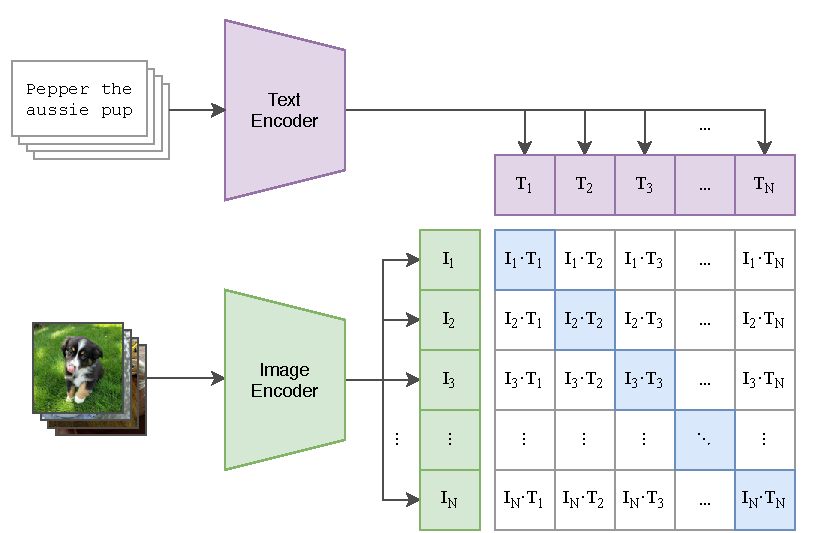
\includegraphics[width=0.45\linewidth]{figures/论文-图6-CLIP-方法.pdf}}
%   \subcaptionbox{CLIP可扩展性分析\label{fig:6-CLIP-Scaling}}
%     {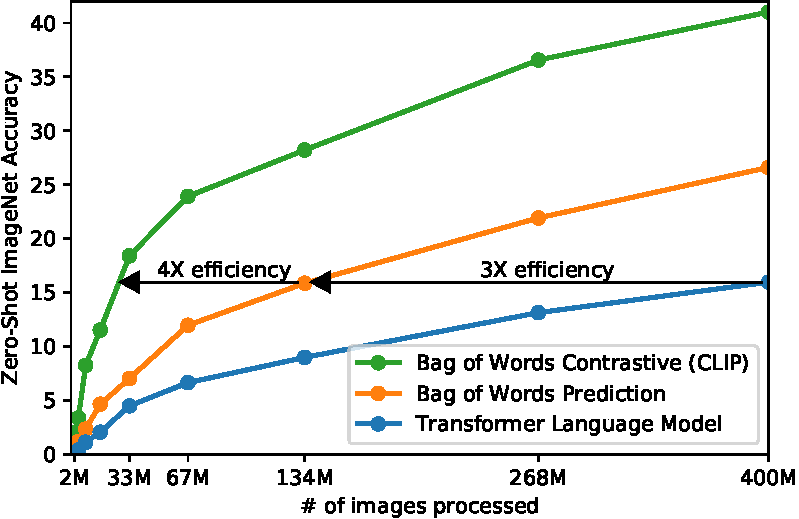
\includegraphics[width=0.45\linewidth]{figures/论文-图6-CLIP-效率.pdf}}
%   \caption{CLIP方法概览与可扩展性对比\cite{radford2021learning}}
%   \label{fig:6-CLIP-Method-Scaling}
% \end{figure}

% % 先不讨论LiT/SigLip/FLIP这些工作
% 在上述的局限性驱动下,以CLIP方法\cite{radford2021learning}为代表的视觉-语言多模态联合预训练方法逐渐被推广开来。如图\ref{fig:5-character-instance}(b)所示,这类方法\cite{radford2021learning,jia2021scaling,pham2023combined}可以看作是基于实例级对比学习的自监督预训练方法\cite{chen2020simple}的扩展。
% 在本文中,统一将这类利用互联网大规模图文配对数据进行实例级对比学习的方法统称为CLIP方法,而其中的代表工作即为OpenAI于2021年提出的CLIP模型\cite{radford2021learning}。
% 相比于字符级联合预训练方法,实例级方法不再要求模型在给定图像的情况下逐字符地预测文本信号,而是将配对的\{图像,文本\}信号视作对同一抽象对象的两种不同的描述方式。
% 实例级预训练方法的核心在于构建一个不同描述的共享表征空间,聚合属于同一对象不同描述的表征,分散属于不同对象不同描述的表征。因此,这种方法建模了图像与文本间的相对关系,不依赖图像与文本一一配对的强假设。
% 如图\ref{fig:6-CLIP-Method}所示,将一组$N$张图片记作$\mathcal{I}=\{I_1,\cdots,I_N\}$,将对应的一组$N$条替代文本记作$\mathcal{T}=\{T_1,\cdots,T_N\}$,记模型参数为$\theta$,实例级视觉-语言多模态联合预训练CLIP方法本质上在最大化如下概率估计:
% \begin{equation}
%     \max_{\theta}\left[\sum_{i=1}^{n}f(I_i,T_i)-\sum_{i\neq j;i,j\in[1,N]}f(I_i,T_j)\right]
%     \label{eq:instance-level}
% \end{equation}
% 其中$f$为某种距离度量方式,在CLIP方法中以视觉表征和语言表征的余弦相似度来表示。

% 从式\eqref{eq:instance-level}可以看出,实例级视觉-语言多模态联合预训练方法不再强调建模单个\{图像,文本\}对之间的对应关系,而是通过$N$个一组配对,对齐图像集合$\mathcal{I}$的表征空间和文本集合$\mathcal{T}$的表征空间。
% 尽管这类方法的监督信息量相比于字符级预训练方法较少,但它对数据质量的信噪比要求更低,更符合互联网大规模\{图像,替代文本\}对的实际特性,因此可以通过有效扩展训练样本数目来确保监督信息量充足。
% 如图\ref{fig:6-CLIP-Scaling}所示,CLIP模型证明这种方法相比于利用弱语义话题标签的弱监督方法有4倍的数据利用效率提升(绿色线与橙色线),而相比于字符级预训练方法则有12倍的数据利用效率提升(绿色线与蓝色线)。
% % 同时,实例级语言监督方法从字符序列长度不同的文本中得到的训练信号信息量一致,不存在某些图像学习不平衡导致的收敛不充分问题,也不存在序列长度不均衡带来的实现效率问题。
% 此外,实例级视觉-语言多模态联合预训练方法直接对齐了视觉表征与语言表征,因此为图文检索、物体识别、模态转换等下游任务提供了重要帮助。
% % 天然提供了一项额外好处:\todo{简单的大规模检索算法和零样本开放集合识别} % 开放集合识别貌似基于回归的办法也可以做。可以提检索简化了识别(把open end的映射问题转为排序问题),对物体检测、语义分割都有帮助
% 综上所述,实例级视觉-语言多模态联合预训练方法具备高效的数据利用效率和大规模扩展的潜力。同时CLIP方法作为一种基于语言监督的视觉模型预训练方法对视觉模型训练研究同样有深刻影响。